\section{Details about Experiments}
\label{more_exp}
Here we discuss more about experiments. The generating process is the following:

\begin{enumerate}
    \item Generate $n$ samples from the uniform distribution on $[-1,1]^d$. Inner points are the ones that are sampled from $[-0.8, 0.8]^d$.
    \item Apply the transformation $f$ to these points to get the samples on the manifold.
    \item Use high dimensional rotation matrix to lift manifold into high dimension and add noise to the samples if needed. 
\end{enumerate}
that is
\begin{align}
    x \in \R^2 \overset{Ax + b}{\longrightarrow} h \in \R^2 \overset{f}{\longrightarrow} y_{small} \in \R^d \overset{Ratation}{\longrightarrow} y \in \R^{48}
\end{align}

For example, setting for swiss roll is 
\begin{align}
    A = \begin{pmatrix}
        (\alpha - \beta)/2 & 0 \\
        0 & h/2 
    \end{pmatrix}, b = \left((\alpha+\beta)/2, h/2 \right), f = \begin{pmatrix}
        h_1 \cos h_1\\ h_2 \\ h_1 \sin h_1
    \end{pmatrix},
\end{align}
the setting for torus is 
\begin{align}
    A = \begin{pmatrix}
        \pi & 0 \\
        0 & \pi 
    \end{pmatrix}, b = \left(\pi, \pi \right), f = \begin{pmatrix}
        (R + r \cos h_2) \cos h_1 \\
        (R + r \cos h_2) \sin h_1 \\
        r \sin h_2
    \end{pmatrix},
\end{align}
the setting for random manifold $1$ is 
\begin{align}
    A = \begin{pmatrix}
            -2.224, & 0.073 \\
            -0.134 & -1.006
    \end{pmatrix}, b = \left(0.124 , 1.403 \right), f = \begin{pmatrix}
        1/(e^{h_1}+1) \\
        \cos h_2 \\
        \sin 2h_2
    \end{pmatrix},
\end{align}
the setting for random manifold $2$ is 
\begin{align}
    A = \begin{pmatrix}
            -1.885 & 0.111 \\
            0.006 & 1.266
    \end{pmatrix}, b = \left(0.370 , -0.457 \right), 
    &f^1 = \begin{pmatrix}
        1/(e^{h_1}+1) \\
        e^{h_2}
    \end{pmatrix}, f^2 = \begin{pmatrix}
        f^1_1 + 0.5 \\
        2 f^1_2
    \end{pmatrix} \\

    &f^3 = \begin{pmatrix}
        f^2_1 \cos f^2_2 \\
        f^2_1 \sin f^2_2
    \end{pmatrix}, f = \begin{pmatrix}
        f^1 \\
        f^3
    \end{pmatrix}
\end{align}

These manifold data are sampled from non uniform distribution on the manifold, but the density is bounded from above and below, which satisfies our assumption.

\subsection{More Experiments about Diffusion Maps}
We frist discuss the DM on the unbounded linear space. For simplicity, we consider $2$ dimensional linear subspace in $\R^3$, i.e. $xOy$ plane, and the Laplacian operator $\Delta$ on it is $-\frac{\partial^2}{\partial x^2} - \frac{\partial^2}{\partial y^2}$. Then for any $a,b \in \R$, $\cos(ax+by)$ is an eigenfunction of $\Delta$ with eigenvalue $a^2 + b^2$. Therefore, its spectrum is continuous, thus we cannot enumerate eigenvalues and eigenfunctions, so DM is not well defined.

If we consider a bounded linear space, i.e. a square, we observe the horseshoe phenomenon, as shown in Figure~\ref{fig:horseshoe}. Selecting the first two coordinates of the DM exhibits the horseshoe phenomenon. However, removing the repeated eigenvector ($\varphi_2$ or $y$--axis) can recover the manifold correctly.
\begin{figure}[H]
  \centering
   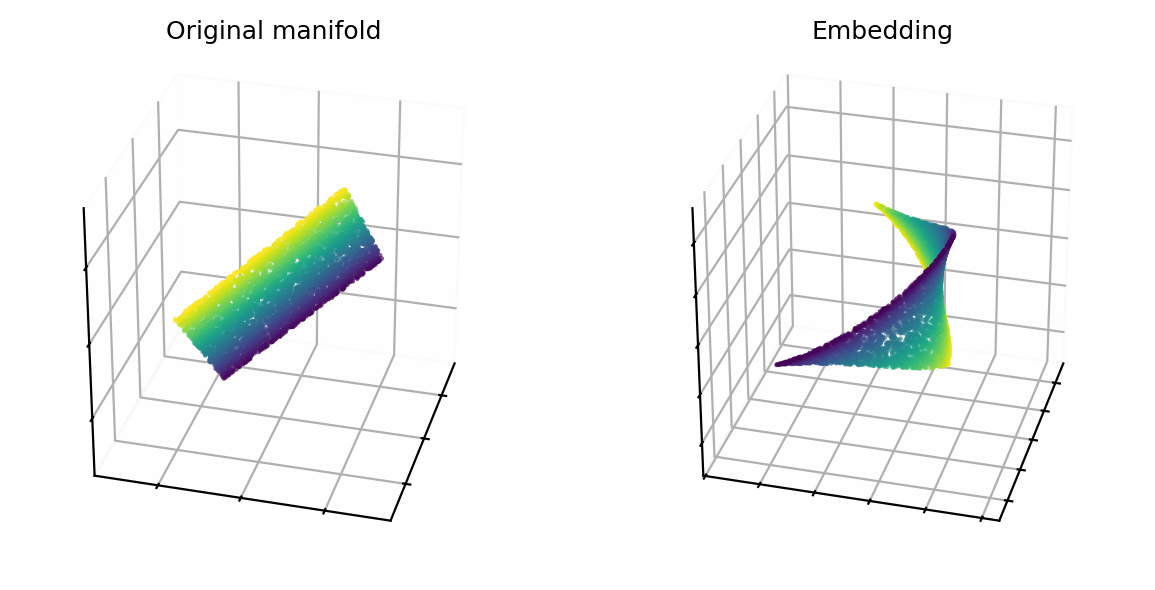
\includegraphics[width=0.8\textwidth]{figures/horseshoe.png}
  \caption{Diffusion maps on a bounded flat manifold exhibit the horseshoe phenomenon. Left: samples from a 2D linear subspace in $\R^3$. Right: the 3D diffusion-map embedding $(\phi_1,\phi_2,\phi_3)$, which bends the flat square into a horseshoe shape rather than recovering the plane.}
  \label{fig:horseshoe}
\end{figure}

\subsection{Experiments about $n$}
Our main theorems are for a family of manifolds, where the geometric quantities are defined independently of any sampling. In practice, a finite point cloud is used and it is only a numerical discretization of such a continuous object. The purpose of this experiment is to show that our estimates exhibit a convergence behavior: as the number of samples $n$ increases, the estimation error decreases steadily toward zero. Such convergence indicates that the estimated quantities genuinely approximate the underlying geometric quantities, which makes the measurements reported in our main experiments meaningful.

We illustrate this on two quantities. For the Riemannian metric, we sample $n$ points from the unit sphere $S^2$ and report the deviation of the estimated metric's singular values $\sigma$ from $1$, measured both on average ($\mathrm{mean}\,|\sigma-1|$) and in the worst case ($\max\,|\sigma-1|$). For the reach, we sample $n$ points from a torus with reach $\tau = 1.5$ and compare the estimate $\hat{\tau}$ against this ground truth. We vary $n \in \{500, 1000, 2000, 5000, 10000\}$, repeat each setting three times, and report the mean together with the min--max range.

\begin{figure}[htbp]
    \centering
    \begin{minipage}[t]{0.48\linewidth}
        \centering
        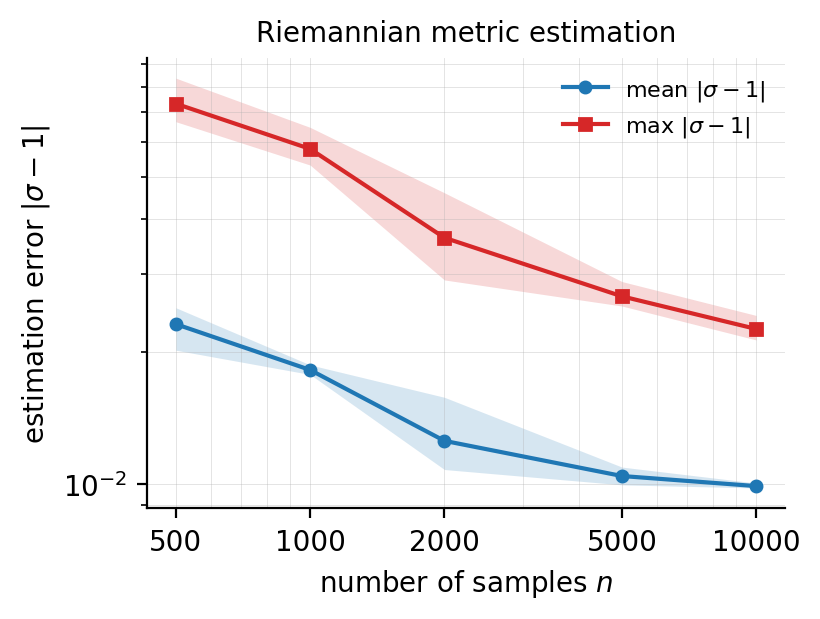
\includegraphics[width=\linewidth]{figures/rmetric.png}
        \caption{Metric estimation error on $S^2$ decreases as $n$ grows}
        \label{fig:metric}
    \end{minipage}%
    \hfill 
    \begin{minipage}[t]{0.48\linewidth}
        \centering
        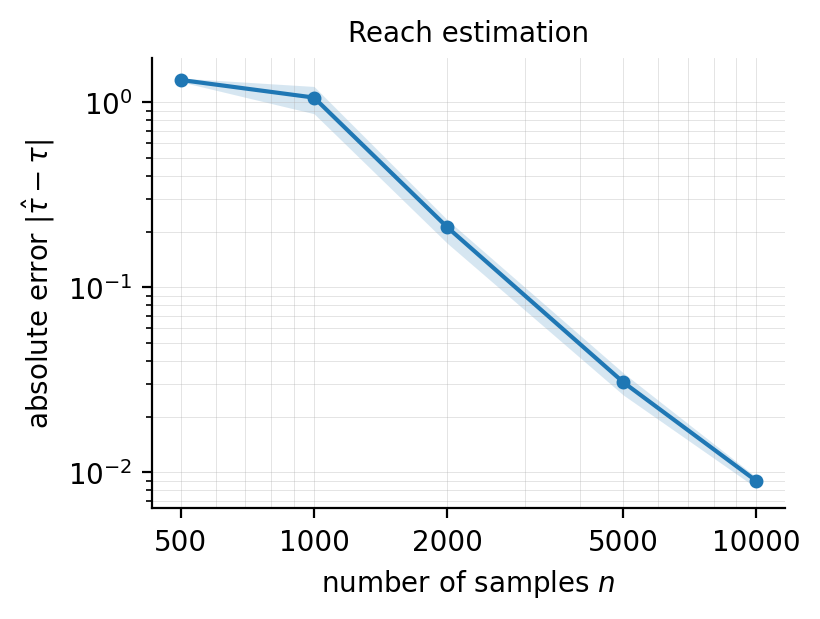
\includegraphics[width=\linewidth]{figures/reach.png}
        \caption{Reach estimation error on a torus ($\tau=1.5$) decreases as $n$ grows.}
        \label{fig:reach}
    \end{minipage}
    \label{fig:total}
\end{figure}

As shown in Figure~\ref{fig:metric} and Figure~\ref{fig:reach}, the estimation error decreases steadily as $n$ grows for both the Riemannian metric and the reach. This convergence confirms that our estimators are consistent in practice and that the measurements reported in our main experiments are meaningful.
